\chapter{Software}

Durante el transcurso de este trabajo se ha dividido el desarrollo del software en varias partes, en las cuales se profundizará a continuación.

\section{Software del Autopiloto}
	
	El autopiloto es la parte del multirrotor que se encarga de generar las acciones de control o comandos, que permitan que el dron llegue a un determinado estado.
	Para generar esas acciones de control, el autopiloto estima el estado de la aeronave en cada instante mediante las lecturas de las IMUs y en función del estado genera las acciones de control pertinentes para mantener la estabilidad de la aeronave. Además el autopiloto que se ha desarrollado cuenta con un interfaz WiFi, por lo que permite enviar y recibir datos del autopiloto a una estación de tierra. A continuación se profundizará en como se han llevado a cabo estas tareas.

\subsection{Estimación del Estado}
	Para estimar el estado, el autopiloto toma las medidas procedentes de las 2 IMUs a través del protocolo I2C con una frecuencia de comunicación de 400KHz.
	Las lecturas del BNO055 proporcionan un estado completo de la aeronave con una frecuencia de refresco de 100Hz. Sin embargo, el MPU9250 nos proporciona medidas relativas a las velocidades angulares y aceleraciones lineales con una tasa de refresco más elevada. Es por esto que se han empleado ambos sensores para conseguir el estado deseado con la mayor precisión y menor tasa de refresco posible.
	
	Con este método se consigue estimar el estado deseado:
	 \begin{equation}
	 	S_t=\big(\underbrace{\varphi,\theta,\psi}_\text{BNO} ,\underbrace{\dot\varphi,\dot\theta,\dot\psi}_\text{MPU} \big)
	 \end{equation}
	consiguiendo minimizar la deriva de la estimación, empleando las lecturas muy estables del BNO055, sin perder la reactividad de las medidas que proporciona el MPU9250.
	
\subsection{Interfaz WiFi}
	Con la intención de poder transmitir datos entre el autopiloto y la estación de tierra se ha diseñado un sencillo protocolo de comunicación WiFi basado en el envió de paquetes de tamaño fijo. El ESP32 cuenta con un sistema operativo en tiempo real (RTOS) el cual se encarga de mantener activa las comunicación WiFi de forma transparente al usuario. La estructura de los paquetes es la siguiente:
	
	\begin{itemize}
		\item \textbf{Autopiloto $\rightarrow$ Estación}: Este paquete contiene 6 datos de tipo \textit{float} (32-bits). Se emplea para enviar la estimación del estado a la aeronave en tiempo real. Esto se emplea para tanto monitorización del desempeño de los algoritmos, como para poder cerrar el bucle de control en la estación base y enviar las acciones de control a la aeronave posteriormente. 
		\item \textbf{Autopiloto $\leftarrow$ Estación}: Este paquete contiene 4 datos de tipo \textit{float} (32-bits) y un dato de tipo \textit{byte}. El dato de tipo \textit{byte} se emplea para controlar el modo de funcionamiento de la aeronave, mientras que los otros 4 datos tienen distintos usos en función del modo:
		
		\begin{itemize}
			\item \textbf{MODO 0} (Desarmado): La aeronave se encuentra ``desarmada'' por lo que los motores no reciben acciones de control. En este modo los demás datos del paquete son irrelevantes.
			
			\item \textbf{MODO 1} (\textit{Off-board}): Las acciones de control son emitidas por la estación de tierra, es decir, la aeronave envía la estimación del estado al ordenador y envía el comando recibido a los variadores. En este modo los datos de tipo \textit{float} del paquete representan los comandos de los motores.
			
			\item \textbf{MODO 2} (\textit{On-board}): El algoritmo de control se ejecuta en la aeronave y se generan las señales de control necesarias a una frecuencia  fijada previamente. En el caso de los controladores PID a bordo, los valores de los 4 datos del paquete permiten variar los valores de las constantes del regulador en tiempo real, lo que facilita el ajuste de las mismas.
		\end{itemize}
		
	\end{itemize}

\subsection{Generacion de comandos \textit{on-board}}
	Para poder maximizar la frecuencia del algoritmo de control y permitir el control de la aeronave sin necesidad de una estación de tierra, los algoritmos de control validados en la simulación se pueden implementar directamente en el autopiloto, fijando previamente la frecuencia a la que se desea que se ejecute el algoritmo. 
	\tb{actualizar en el momento}
	En este trabajo se han implementado a bordo dos algoritmos de control distintos: un regulador PID clásico y un regulador PID en cascada.
	
\section{Software de la estación}

La estación base se ha empleado tanto como para la simulación del entorno, permitiendo diseñar y probar algoritmos de control de forma segura, como para monitorizar los rendimientos de estos algoritmos o incluso, aprovechando la mayor capacidad computacional de estas estaciones, ejecutar los algoritmos de control y aprendizaje por refuerzo en estas.
A continuación se profundizará con más detalle en la implementación de estas herramientas. 


\subsection{Entorno de simulación}

En cualquier proyecto de robótica es conveniente contar con un entorno de simulación que permita realizar pruebas en distintas situación de forma sencilla y rápida, sin necesidad de tener ni modelo real, ni el entorno concreto en el que quieras probar tu robot. Cuando se trabaja con drones, la simulación pasa de ser conveniente a ser muy necesaria. Ésto es debido a la peligrosidad intrínseca de estas aeronaves, ya que, cuentan con hélices afiladas que giran a gran velocidad.

%Es por esto que es necesario contar con un entorno de simulación en el que se puedan probar los algoritmos de control antes de llevarlos a la realidad, con el objetivo de minimizar los riesgos de estas pruebas.Si a todo esto se le añade la experimentación con algoritmos de aprendizaje por refuerzo e inteligencia artificial, la simulación y entrenamiento previos se hacen imprescindibles 

Debido a la naturaleza del apredizaje por refuerzo, este requiere de la interacción de un agente con un entorno para que el agente aprenda que acciones son las que debe tomar en cada estado. Esto significa que al comienzo del entrenamiento el agente realiza acciones aleatorias para poder explorar cuales son las que le proporcionan una recompensa mayor.

Debido a esta forma de explorar, el agente requiere de una gran cantidad de pruebas, de ensayo y error, hasta que consigue aprender, por lo que no es conveniente realizar todas estas iteraciones en un modelo real.

Por estas razones se necesita de un entorno de simulación para poder validar los algoritmos y poder generar modelos entrenados en simulación sin deteriorar el equipo real. Además el entorno en simulación te permite entrenar distintos agentes simultáneamente y reducir los tiempos de entrenamiento.

Para el entorno de simulación nos hemos basado en Gym \tb{citar},una librería escrita en Python y desarrollada por la compañía OpenAI, que permite desarrollar y comparar algoritmos de aprendizaje por refuerzo. Esta librería te permite generar un entorno con el cual interactúe el agente, sin importar la implementación de éste, permitiendo comparar el rendimiento de distintos agentes sobre el mismo entorno.
\tb{IMAGEN GYM}

\tb{revisar} Como entorno de simulación se ha partido de GymFC, desarrollado por William Koch et al. \cite{koch2019reinforcement}.
Este entorno de simulación utiliza Gazebo 9, un entorno de simulación 3D de código abierto ampliamente utilizado en el campo de la robótica. En este entorno se simula el comportamiento de un multirrotor, concretamente el de un modelo del cuadricóptero IRIS.
\tb{imagen GYMFC}

Para acercar la simulación a la configuración de los experimentos que se realizarían posteriormente en la plataforma real, se han realizado algunas modificaciones sobre el modelo predeterminado de la aeronave:

\begin{enumerate}
	\item Se ha modificado la forma de anclaje del dron. Originalmente el dron se encontraba anclado entorno a una articulación situada en su centro de gravedad. Esto permitía que el peso de la aeronave apenas tuviera influencia a la hora de rotar la aeronave, todo el peso estaba sustentado por la articulación, lo cual no se asemeja con los bancos de pruebas que se han diseñado. En estos bancos de prueba el anclaje se encuentra desplazado con respecto al centro de gravedad, por lo que cuanto mayor sea el valor de los ángulos $\varphi$ y $\theta$ mayor es la influencia del peso en el par necesario para estabilizar la aeronave. Es por esto que se ha desplazado la articulación del centro de gravedad y se ha conectado a la aeronave mediante una unión rígida, asemejando así el entorno de simulación al entorno de pruebas real.
	\item Se ha modificado parámetros dinámicos de la aeronave. Los parámetros que mayor discrepancia tenían entre la simulación y el mundo real eran principalmente los parámetros inerciales. Tanto la masa como los momentos de inercia del cuadricóptero eran mucho inferiores a los de la aeronave real. Esto se manifestaba principalmente cuando al hacer pruebas con los algoritmos PID el comportamiento simulado no se parecía con el real, por ejemplo en simulación un regulador P era capaz de estabilizar al sistema, mientras que en la realidad un regulador P era inestable de por sí y requería de las acciones derivativa e integral para conseguir estabilizarlo.
\end{enumerate}

%Para acercar la simulación a la configuración de los experimentos que se realizarían posteriormente en la plataforma real, se ha situado una articulación en su centro de gravedad que fija la posición de su centro pero permite rotar el numero de grados de libertad que se predefina.


 \subsection{Agente (generación de comandos)}
 
 Siguiendo con la terminología del aprendizaje por refuerzo se va a denominar agente al encargado de generar las acciones de control. En el caso de los reguladores PID clásicos el agente hace la función de los reguladores.

Para probar distintos agentes con distintos algoritmos se han empleado la implementación de los algoritmos \textit{state of the art}, del repositorio de GitHub \textit{Stable-Baselines} \cite{stable-baselines}. Inicialmente se comenzó empleando las \textit{Baselines} de OpenAI \cite{OpenAIbaselines} pero se decidió cambiar a las \textit{Stable Baselines} por la limpieza del código y la facilidad para realizar experimentos con diversos algoritmos e hiperparámetros.

\tb{¿hablo un poco sobre transfer learning?}


\subsection{Interfaz Estación-Autopiloto}

Para las pruebas reales se ha empleado ROS (Robotic Operative System) Melodic para gestionar la comunicación WiFi con la aeronave y la comunicación con el agente. Para esto se emplea la estructura de \textit{topics}: un \textit{topic} se emplea para enviar datos a la aeronave y otro \textit{topic} publica los datos recibidos por ésta. De esta manera se pueden utilizar las herramientas de ROS para poder monitorizar el proceso además de aprovechar la estructura de \textit{topics} para poder intregrar código escrito en distintos lenguajes de forma sencilla.

\begin{figure}[htb!]
	\centering
	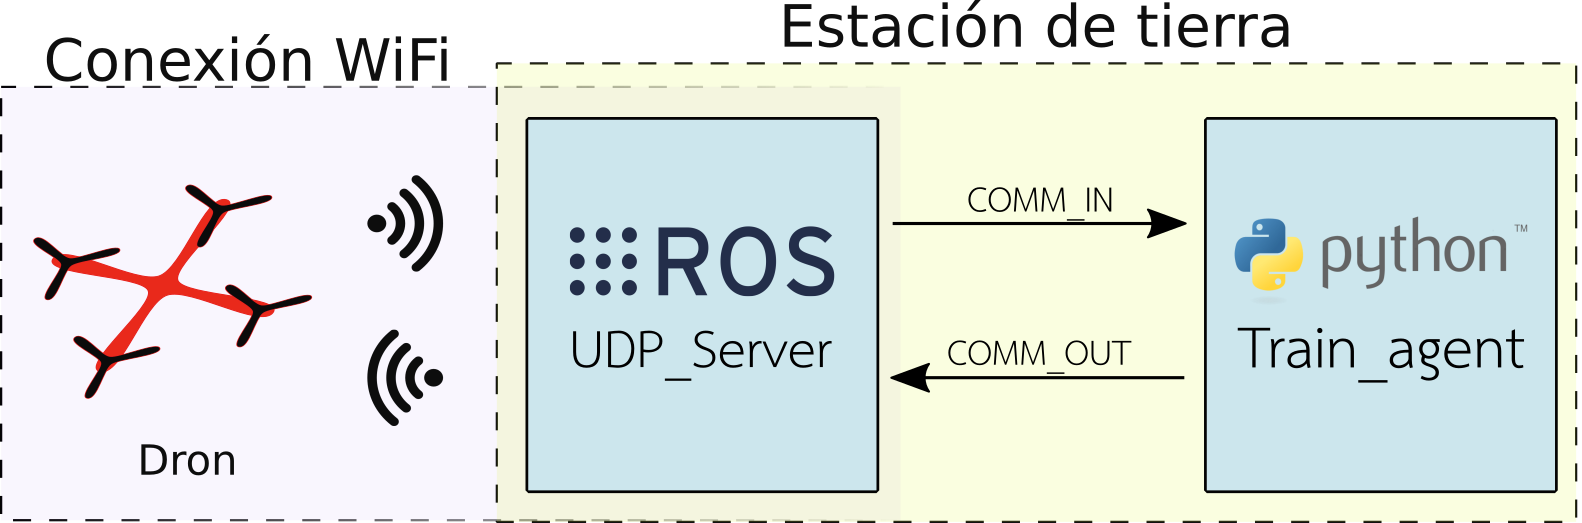
\includegraphics[width=0.9\textwidth]{software/Arquitectura}
	\caption{Esquema interfaz Estacion-Autopiloto}
	\label{hardware:esc_explicacion}
\end{figure}





\section{Descripción del equipo}
Para el desarrollo del trabajo se ha empleado un portatil MSI-GE62 empleando Windows 10 para el desarrollo CAD y Ubuntu 18.04 LTS para el resto de las tareas. El equipo cuenta con 16GB de RAM DDR4, un procesador Intel i7-6700HQ de 8 núcleos a 2.60GHz y una GPU GeForce GTX 970M con 3GB de memoria dedicada.

